
\subsection{Clasificación de la criptografía}

  La criptografía puede clasificarse de forma histórica en dos categorías,
  la criptografía clásica y la criptografía moderna. La criptografía clásica
  es aquella que se utilizó desde la antigüedad, teniéndose registro de su
  usado desde hace más 4000 años por los egipcios, hasta la mitad del siglo
  XX. En esta los métodos utilizados para cifrar eran variados, pero en su
  mayoría usaban la transposición y la sustitución, además de que la mayoría
  se mantenían en secretos. Mientras que la criptografía moderna es la que
  se inició después la publicación de la \textit{Teoría de la información}
  por Claude Elwood Shannon, dado que esta sentó las bases matemáticas para
  la criptología en general.

  Una manera de clasificar es de acuerdo a las técnicas y métodos empleados
  para cifrar la información, esta clasificación se puede observar en la
  siguiente figura.

  \begin{figure}[H]
    \begin{center}
      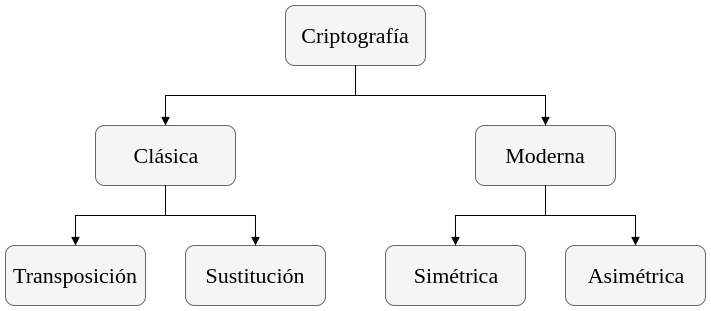
\includegraphics[width=0.75\linewidth]
        {contenidos/antecedentes/intro/img/clasificacion_cripto.png}
      \caption{Clasificación de la criptografía.}
    \end{center}
  \end{figure}

  Adentrándose en la clasificación de la criptografía clásica, se tienen los
  cifrados por transposición, los cuales se basan en técnicas de permutación
  de forma que los caracteres de la información en claro se reordenen
  mediante algoritmos específicos, y los cifrados por sustitución, que
  utilizan técnicas de modificación de los caracteres por otros
  correspondiente a un alfabeto específico para el cifrado.

  En cuanto a la criptografía moderna, esta tiene dos vertientes, la
  criptografía simétrica o de llave secreta y la asimétrica o de llave
  pública. Hablando de la primer vertiente, se puede decir que es aquella
  que utiliza un modelo matemático para cifrar y descifrar un mensaje
  utilizando únicamente una llave que permanece secreta.

  \begin{figure}[H]
    \begin{center}
      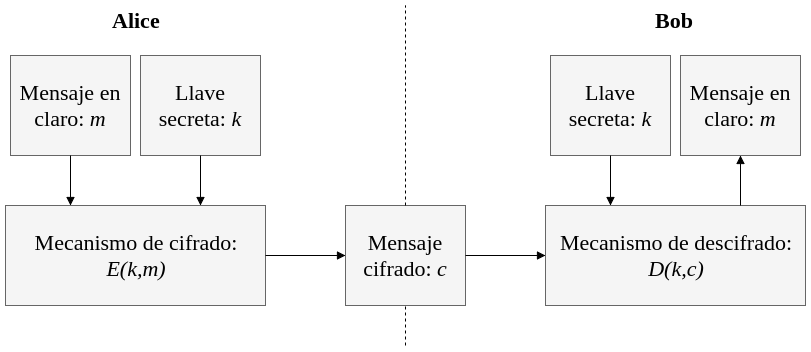
\includegraphics[width=0.8\linewidth]
        {contenidos/antecedentes/intro/img/cripto_simetrica.png}
      \caption{Canal de comunicación con criptografía simétrica.}
    \end{center}
  \end{figure}

  En la figura anterior se puede observar el proceso para establecer una
  comunicación segura por medio de la criptografía simétrica. Primero, tanto
  Alice como Bob deben de establecer una llave única y compartida $k$, para
  que después, Alice, actuando como el emisor, cifre un mensaje $m$ usando
  la llave $k$ por medio del algoritmo de cifrado $E(k,m)$ para obtener el
  mensaje cifrado $c$ y enviárselo a Bob. Posteriormente Bob, como receptor,
  se encarga de descifrar $c$ con ayuda de la llave $k$ por medio del
  algoritmo de descifrado $D(k,c)$ para obtener el mensaje original $m$.

  Entre los beneficios de este tipo de criptografía está su utilidad para
  cifrar archivos personales, su relativa facilidad de uso y para garantizar
  la confidencialidad e integridad debido al uso de una llave, y su rapidez,
  pero en contraparte, su uso genera problemas para organizar y compartir
  las llaves secretas de una forma segura y eficiente.

  Ahora, adentrándose en la criptografía asimétrica, se tiene que su idea
  principal es el uso de 2 llaves distintas para cada persona, una llave
  pública para cifrar que esté disponible para cualquier otra persona, y una
  llave privada para descifrar, que se mantiene disponible solo para su
  propietario.

  El proceso para establecer una comunicación segura por medio de este tipo
  de criptografía es el siguiente: primero, Alice nuevamente como el emisor,
  cifra un mensaje $m$ con la llave pública de Bob $pk$ usa el algoritmo de
  cifrado $E(pk,m)$ para obtener $c$ y enviarlo. Después Bob como receptor,
  se encarga de descifrar $c$ por medio del algoritmo de descifrado
  $D(sk,c)$ haciendo uso de su llave privada $sk$. Este proceso se refleja
  gráficamente el la siguiente figura.

  \begin{figure}[H]
    \begin{center}
      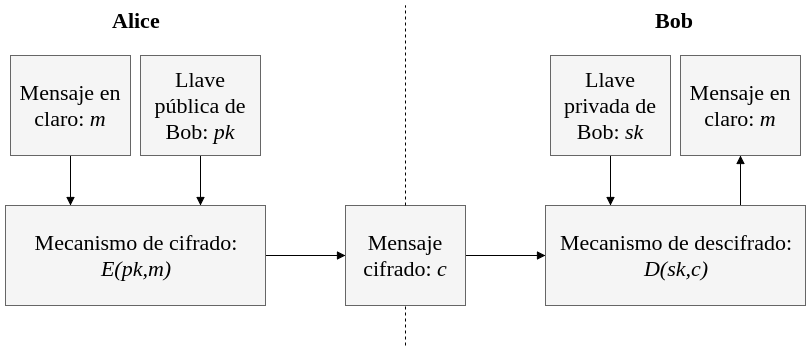
\includegraphics[width=0.8\linewidth]
        {contenidos/antecedentes/intro/img/cripto_asimetrica.png}
      \caption{Canal de comunicación con criptografía asimétrica.}
    \end{center}
  \end{figure}

  Entre los uso que se le da a esta criptografía está el mantener la
  distribución de llaves privada segura, y establecer métodos que garantizan
  la autenticación y el no repudio, como por ejemplo en las firmas y
  certificados digitales.
